\documentclass[a4paper,11pt,dvipdfmx]{jsarticle}

\usepackage{bm}
\usepackage[dvipdfmx]{graphicx}
\usepackage[dvipdfmx]{color}
\usepackage{ascmac}
\usepackage{amsmath}
\usepackage{amssymb}
\usepackage{siunitx}
\usepackage{otf}
\usepackage[dvipdfmx]{graphicx}
\pagestyle{plain}
\usepackage{float}
\usepackage[dvipdfmx]{hyperref}
\usepackage{pxjahyper}
\usepackage{here}
\usepackage{titlesec}
\titleformat*{\section}{\LARGE\bfseries}
\titleformat*{\subsection}{\normalsize\bfseries}
\usepackage{url}
\usepackage[table,xcdraw]{xcolor}
\hypersetup{% hyperrefオプションリスト
setpagesize=false,
 bookmarksnumbered=true,%
 bookmarksopen=true,%
 colorlinks=true,%
 linkcolor=blue,
 citecolor=blue,
}

\begin{document}
\renewcommand\thefootnote{\arabic{footnote})}
\newpage
\subsection{原子核半径推定の理論}
前節では本実験において重要な物理量である微分散乱断面積について議論したが、本節ではそれらの議論を元に、本研究の目的である、炭素原子核半径の推定を行うのに必要な理論について論ずることにする。
\subsubsection{最近接距離と原子核半径}
3\;MeVに加速された陽子が標的原子核の中心までどれだけ近づけるのか考える。
式\eqref{eq:saikinsetu}に標的の原子番号$Z$、入射陽子のエネルギー$E=$\;3\;MeV\;$=4.8\times10^{-13}\;$J\,を代入することで最近接距離$r_{min}$を求められる。
\begin{equation}
    r_{min}=\frac{Ze^{2}}{4\pi\varepsilon_{0}E}
    \label{eq:saikinsetu}
\end{equation}

次にターゲットの原子核半径を求める。原子核半径$R$は質量数$A$の1/3乗に比例することが分かっており、以下の式\eqref{eq:radius}で表される。\footnote{本来は近似式であるが、本研究では等式として扱う。}ただし、水素の原子核半径は陽子半径と等しいとみなせるので、式\eqref{eq:radius}には従わない。
\begin{equation}
    R=1.3\times A^{\frac{1}{3}}
    \label{eq:radius}
\end{equation}

表\ref{table:gensi}に各標的ごとに計算された最近接距離と原子核半径を示す。

\begin{table}[htbp]
 \centering
  \begin{tabular}{clll}
   \hline 
   \  & \,Au & \;\,C & \;\,H \\
   \hline \hline
   最近接距離(fm) & 38.7 & 2.94 & 0.49 \\
   原子核半径(fm) & 7.56 & 2.97 & 0.88 \\
   \hline    
  \end{tabular}
  \caption{最近接距離と原子核半径}
   \label{table:gensi}
\end{table}

表\ref{table:gensi}から、炭素原子核と水素原子核(陽子)についてはCoulomb力による散乱だけでなく、核力による散乱を考慮する必要があると分かる。

\subsubsection{炭素の原子核半径}
以上の議論から、炭素原子核についてCoulomb力による散乱と核力による散乱の場合の微分散乱断面積を比較したものが図\ref{fig:hikaku}になる。

図\ref{fig:hikaku}において、青色の線は核力、赤色の線はCoulomb力、水色の線はCoulomb力と核力を足し合わせたものである。

図\ref{fig:hikaku}から、散乱角$80^{\circ}$付近から核力による影響がCoulomb力による影響より大きくなり、より大角度では核力による影響が支配的になると言える。
よって、大角度での微分散乱断面積の測定値から炭素の原子核半径を推定することができる。
\begin{figure}[htbp]
\centering
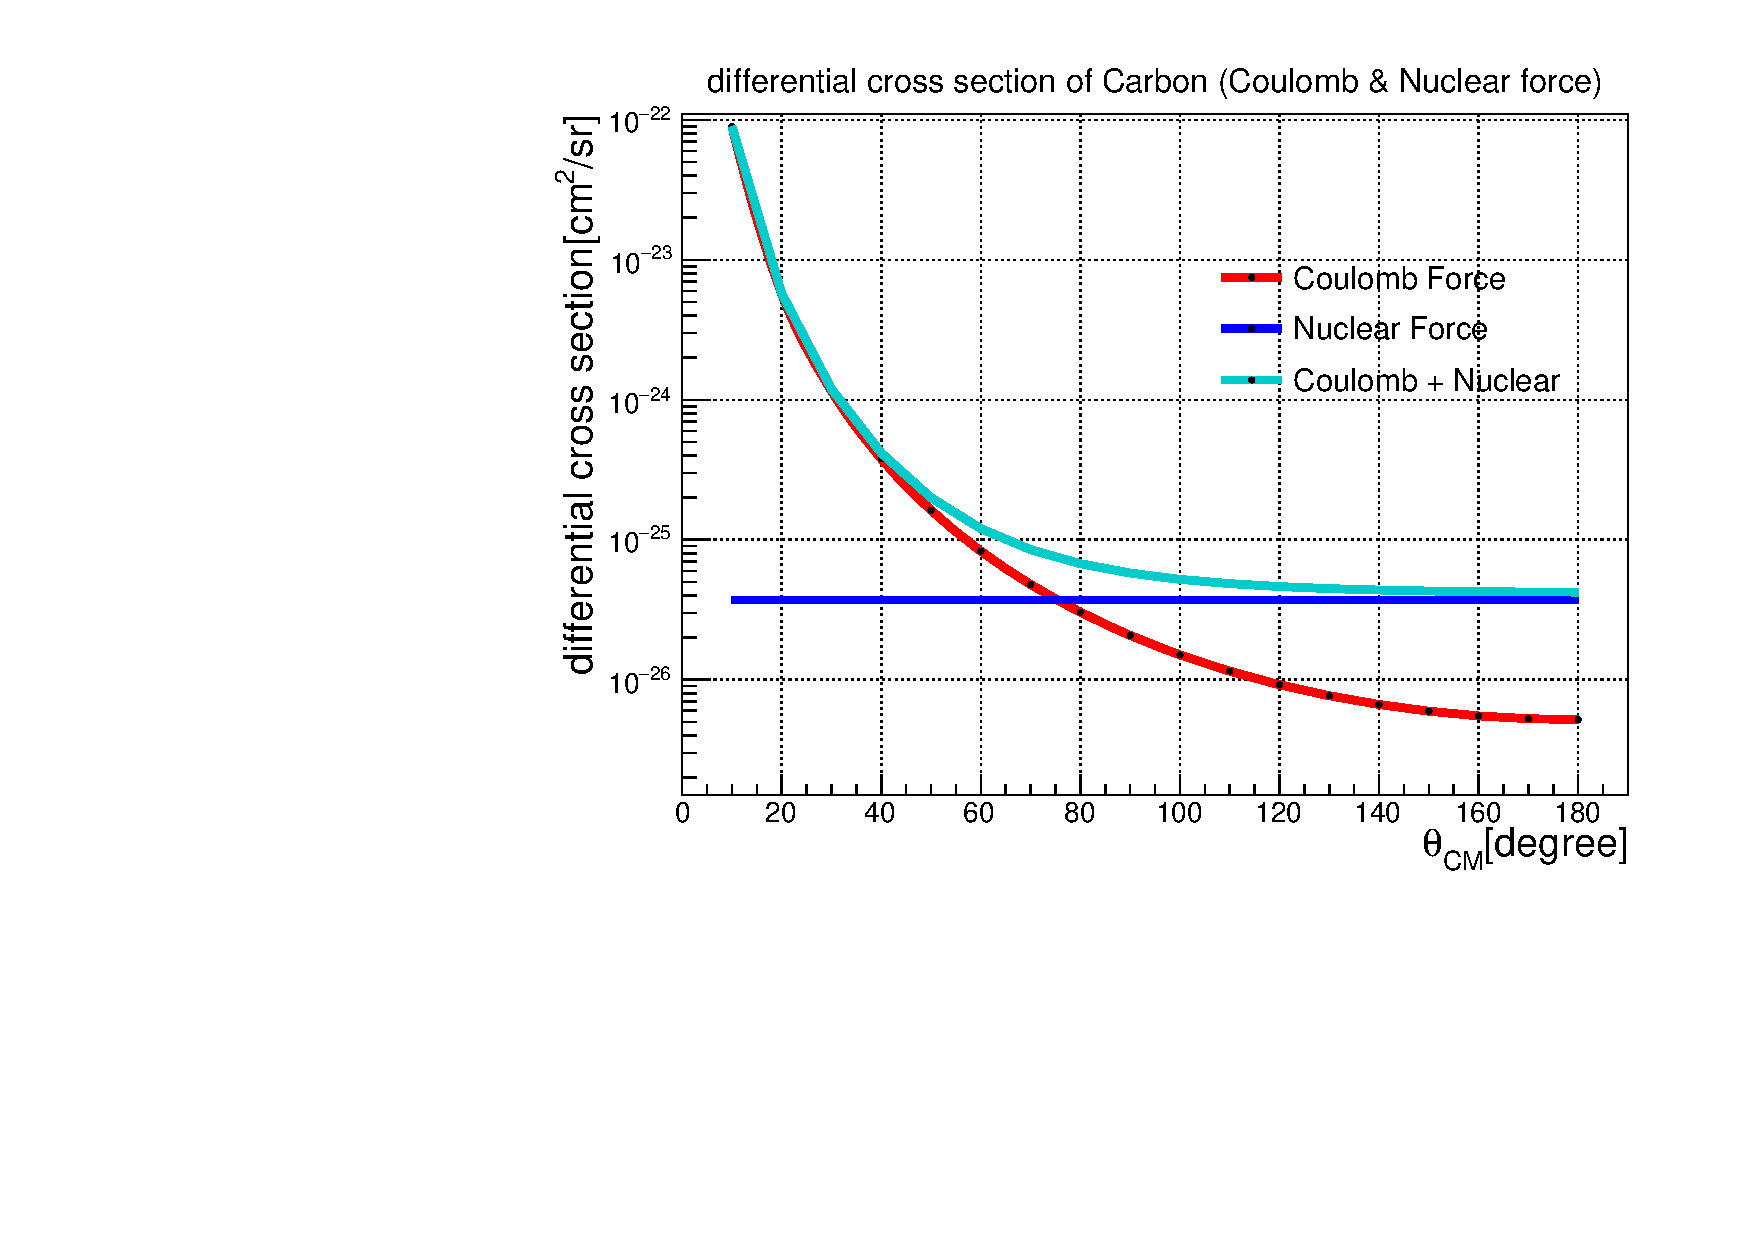
\includegraphics[width=9cm]{picture/radiustheory/kakutei.pdf}
\caption{炭素の微分散乱断面積}
\label{fig:hikaku}
\end{figure}

\end{document}